\section{17.05.2018, 24.05.2018 - R Turotium}
- Führen Sie die im Tutorium: https://www.tutorialspoint.com/r/r\_web\_data.htm angegebenen Unterpunkte zu R Data Interfaces, R Charts \& Graphs und R Statistics Examples aus.
- Wenden Sie anschließend die Beispiele aus den Tutorien auf Ihre eigenen Daten an

\subsection{Kurzdarstellung der Aufgabenstellung}
Es sollen Daten aus einem beliegen Bereich gewählt werden und in einer Datenbank abgelegt werden. Auf die Datenbank soll mit R zugriffen werden um die Daten analysieren zu können.
\subsection{Lösung}
- gewählter Datensatz: https://www.kaggle.com/harlfoxem/housesalesprediction
- beinhaltet Hausverkaufsdaten von Häusern in King County (USA) im Jahre 2014
- Daten wurden in MS-Access (C:/users/admin/documents/DATA\_DB.mdb) mit der CSV-Importfunktion eingelesen

\begin{figure}[!htb]
        \begin{minipage}{1\textwidth}
                \centering
                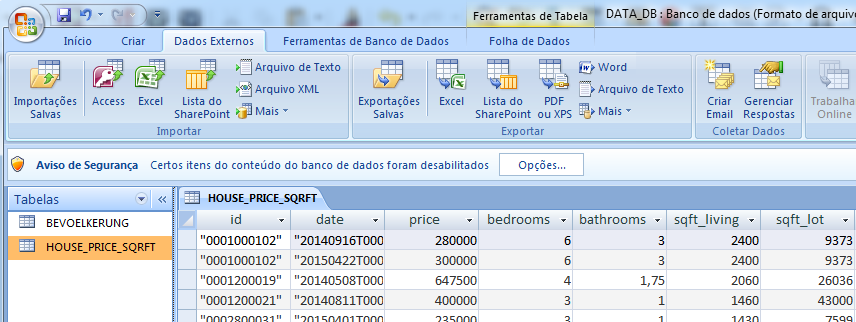
\includegraphics[width=0.90\textwidth]{pics/tutor1.png}\par\vspace{0cm}
                \caption{Import MS-Access}
                \label{fig:tutor1}
        \end{minipage}
\end{figure}

Für die analyse wurde nur R gestartet und folgende Aktionen/Befehle ausgeführt:
Installieren RODBC Package:
\begin{lstlisting}
install.packages("RODBC")
\end{lstlisting}
        Aufrufen Package RODBC:
\begin{lstlisting}
library(RODBC)
\end{lstlisting}
Zuweisen Genutzten Datenbank auf (abgelegt in R source Ordner)
\begin{lstlisting}
channel <- odbcConnectAccess("DATA\_DB.mdb")
\end{lstlisting}

Zweisen der Datentabelle auf Objekt:
\begin{lstlisting}
data = sqlQuery(channel ,paste('SELECT * FROM HOUSE\_PRICE\_SQRFT'))
\end{lstlisting}

Anzeigen der ersten sechs Zeilen der Tabelle/Objekt
\begin{figure}[!htb]
        \begin{minipage}{1\textwidth}
                \centering
                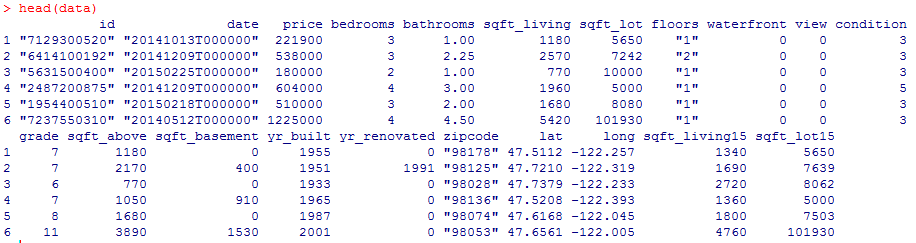
\includegraphics[width=0.90\textwidth]{pics/tutor2.png}\par\vspace{0cm}
                \caption{Anzeigen der Zeilen}
                \label{fig:tutor2}
        \end{minipage}
\end{figure}

Analyse Histogram Preis:
\begin{lstlisting}
hist(data$price,xlab = "price",col = "green",border = "red"
\end{lstlisting}

\begin{figure}[!htb]
        \begin{minipage}{1\textwidth}
                \centering
                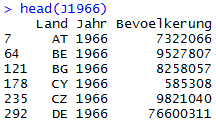
\includegraphics[width=0.90\textwidth]{pics/tutor3.png}\par\vspace{0cm}
                \caption{Analyse Histogramm}
                \label{fig:tutor3}
        \end{minipage}
\end{figure}

Datensatz auf Preise bis maximal 1mio reduzieren:
\begin{lstlisting}
data = sqlQuery(channel ,paste('SELECT * FROM HOUSE_PRICE_SQRFT                 WHERE PRICE < 1000001'))
\end{lstlisting}

        Neues Histogramm ausführen
\begin{lstlisting}
hist(data$price,xlab = "price",col = "green",border = "red")
\end{lstlisting}

\begin{figure}[!htb]
        \begin{minipage}{1\textwidth}
                \centering
                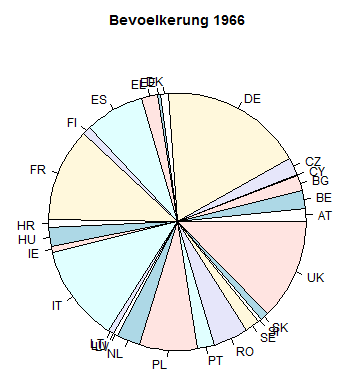
\includegraphics[width=0.90\textwidth]{pics/tutor4.png}\par\vspace{0cm}
                \caption{Weiteres Histogramm}
                \label{fig:tutor4}
        \end{minipage}
\end{figure}

Abfrage minimum Preis in der Datei:
\begin{figure}[!htb]
        \begin{minipage}{1\textwidth}
                \centering
                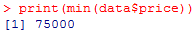
\includegraphics[width=0.90\textwidth]{pics/tutor4-1.png}\par\vspace{0cm}
                \caption{Abfrage Preis}
                \label{fig:tutor4-1}
        \end{minipage}
\end{figure}

Boxplot (Wohnraufgrößen Variation pro Baujahr)
\begin{lstlisting}
boxplot(sqft_living ~ yr_built, data = data, xlab = "YEAR BUILT",+    ylab = "SQFT_LIVINV", main = "SQFT PER YEAR OF CONSTRUCTION")
\end{lstlisting}

\begin{figure}[!htb]
        \begin{minipage}{1\textwidth}
                \centering
                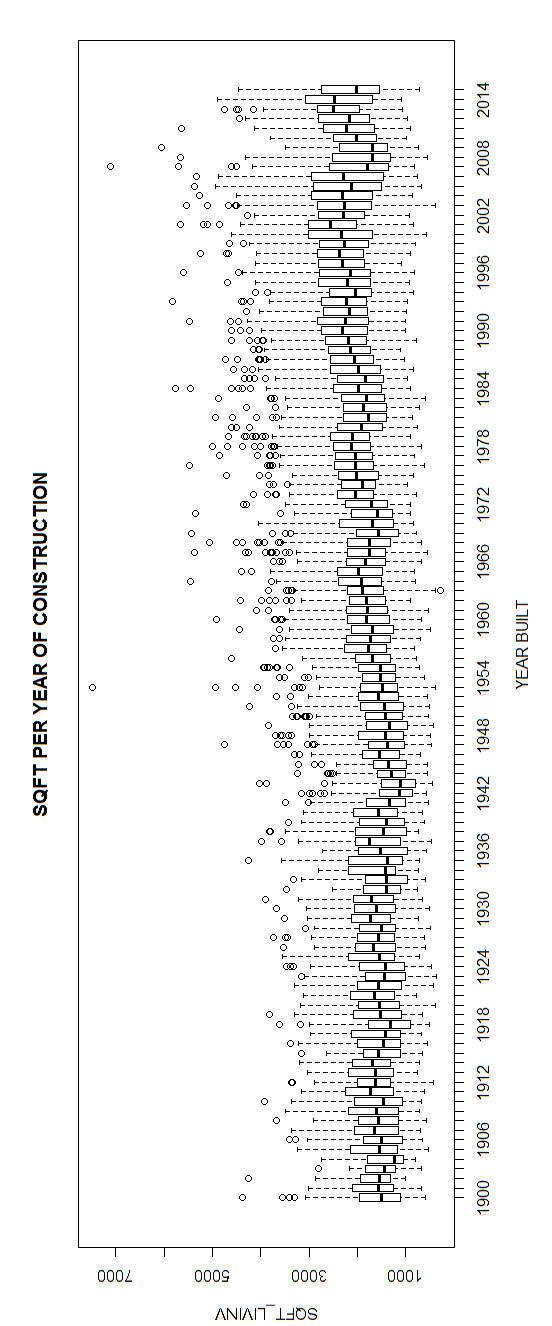
\includegraphics[width=0.90\textwidth]{pics/tutor5.png}\par\vspace{0cm}
                \caption{Boxplot SQFT per year of construction}
                \label{fig:tutor5}
        \end{minipage}
\end{figure}

Erstellen von SCATTER PLOT MATRIX:
\begin{lstlisting}
pairs(~price+sqft_living+sqft_lot,data = data,  +    main = "Scatterplot Matrix")
\end{lstlisting}

\begin{figure}[!htb]
        \begin{minipage}{1\textwidth}
                \centering
                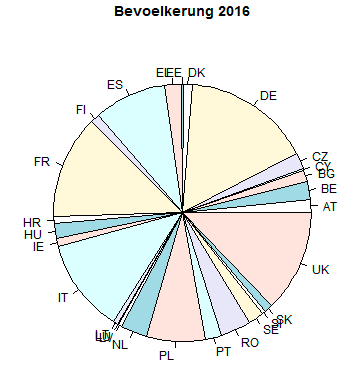
\includegraphics[width=0.90\textwidth]{pics/tutor6.png}\par\vspace{0cm}
                \caption{Scatterplot}
                \label{fig:tutor6}
        \end{minipage}
\end{figure}

- multiple lineare Regression (Price in Abängigkeit Sqft\_Living und Sqft\_Loft)

Installation und Öffnung der relevanten Daten
\begin{lstlisting}
install.packages("caret")
install.packages("ggplot2")
install.packages("lattice")
library(caret)
\end{lstlisting}

Verwendung der Daten in der variable „data“

\begin{figure}[!htb]
        \begin{minipage}{1\textwidth}
                \centering
                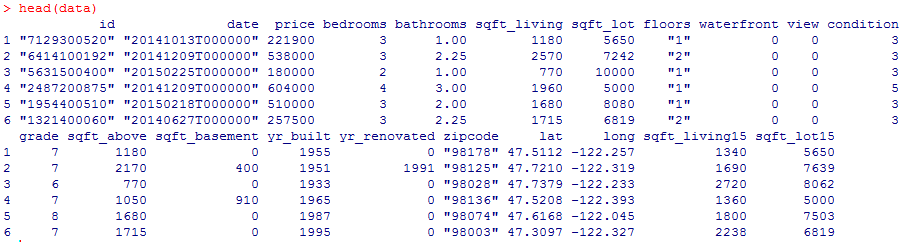
\includegraphics[width=0.90\textwidth]{pics/tutor7.png}\par\vspace{0cm}
                \caption{Variablenverwendung}
                \label{fig:tutor7}
        \end{minipage}
\end{figure}

Verwendung Modell für multiple lineare Regression mit allen mathematisch        vorstellbar relevanten spalten
\begin{lstlisting}
model <-lm(price~bedrooms+bathrooms+sqft_living+sqft_lot+waterfront+    view+condition+grade+sqft_above+sqft_basement+yr_built+yr_renovated,    data = data)
\end{lstlisting}

        Ausgabe des berechneten Modells:

\begin{figure}[!htb]
        \begin{minipage}{1\textwidth}
                \centering
                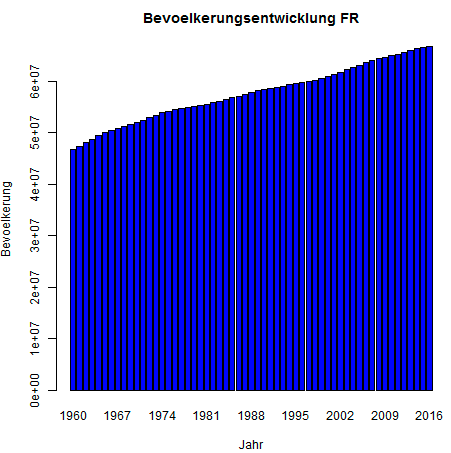
\includegraphics[width=0.90\textwidth]{pics/tutor8.png}\par\vspace{0cm}
                \caption{Ausgabe Berechnungsmodell}
                \label{fig:tutor8}
        \end{minipage}
\end{figure}





\subsection{Aufteilung der Aufgaben im Team}
Alle Aufgabenpunkte wurden gemeinsam bearbeitet
\subsection{Darstellung der benutzen Werkzeuge und Systeme}
\subsubsection*{Entwurfswerkzeug}
MS-ACCESS
\subsubsection*{Entwicklungsumgebung}
R (32bit Version da MS-ACCESS 32bit Version ansonsten Verbindung in der Form nicht möglich)

